\section{梯度, 散度,
和旋度}

前面我们算是过了遍向量的最基本的概念以及运算,
那么有没有关于向量的微积分呢?

\subsubsection{梯度}

考虑三维欧氏空间 \(\mathbb{R}^3\) 中的情况,
如果我们有一个多变量函数/标量场 \(f(x,y,z)\),
相当于把坐标的三个参数映射到一个标量 (暂时先只考虑实变函数):
\(\mathbb{R}^3\rightarrow\mathbb{R}\).

在【023】中, 我们发现, 多变量函数可以分别对各个变量求偏导,
而偏微分和全微分的关系是\footnote{注意, 本篇中有大量忽略函数变量的标记,
  即类似 f=f(x), 请自行脑补全缺失的部分.} \[
\mathrm{d}f=\frac{\partial f}{\partial x}\mathrm{d}x+\frac{\partial f}{\partial y}\mathrm{d}y+\frac{\partial f}{\partial z}\mathrm{d}z.
\] 令 \(\{\hat{\imath},\hat{\jmath},\hat{k}\}\)
分别为平行于三个坐标轴的单位向量, 利用它们的正交归一性,
上式可以重新写作一个点乘的形式 (复习【025】): \[
\mathrm{d}f=\left(\frac{\partial f}{\partial x}\hat{\imath}\right)\cdot\left(\mathrm{d}x\hat{\imath}\right)+\left(\frac{\partial f}{\partial y}\hat{\jmath}\right)\cdot\left(\mathrm{d}y\hat{\jmath}\right)+\left(\frac{\partial f}{\partial z}\hat{k}\right)\cdot\big(\mathrm{d}z\hat{k}\big).
\] 令 \[
\mathrm{d}\boldsymbol{r}:=\mathrm{d}x\hat{\imath}+\mathrm{d}y\hat{\jmath}+\mathrm{d}z\hat{k},
\] 即向量的线元, 再令 \[
\boxed{\nabla f:=\frac{\partial f}{\partial x}\hat{\imath}+\frac{\partial f}{\partial y}\hat{\jmath}+\frac{\partial f}{\partial z}\hat{k},}
\] 这个 \(\nabla f\) 便叫作标量场 \(f\) 的\textbf{梯度} (gradient).
于是有 \[
\mathrm{d}f=\nabla f\cdot \mathrm{d}\boldsymbol{r}.
\] 利用点乘的性质, \[
\mathrm{d}f=|\nabla f||\mathrm{d}\boldsymbol{r}|\cos\theta,
\] 其中 \(\theta\) 是梯度向量和线元向量之间的夹角. 考虑线元
\(\mathrm{d}\boldsymbol{r}\) 的大小不变但方向可以改变的情况,
在任意某一点 \((x,y,z)\) 上, 标量场的全微分 \(\mathrm{d}f\)
最大值应该发生在当 \(\theta=0\) (即\(\cos\theta=1\)),
这时线元向量和梯度向量方向一致, 或者说``沿着''梯度向量; 沿着梯度的方向,
全微分取到最大值, 意味着在这个方向上, 标量场本身变化得最快.

\begin{newquote}
于是在最优化 (optimization) 等数据科学中, 利用梯度的这一性质,
便有梯度下降法 (Gradient-Descent) 用来找局域最值 (local extrema).

其思路是: 数值 (numerical) 计算里, 有时为了计算上的便捷, 我们不求
\(|\nabla f|=0\) 的解析解; in stead, 我们知道在最值处,
就如一元微积分最值处导数为零一样, 梯度是零向量, 于是给定一个起点,
我们不断沿着梯度的方向前进, 直到梯度的大小变为零,
那么我们便到了局域的最值处.
\end{newquote}

那么 \(\nabla\) 这个符号呢, 念做 nabla, 就定义为 \[
\boxed{\nabla:=\frac{\partial}{\partial x}\hat{\imath}+\frac{\partial}{\partial y}\hat{\jmath}+\frac{\partial}{\partial z}\hat{k}.}
\] 当然, 这是在三维欧氏空间中, 使用笛卡尔坐标系时的形式, 在其他坐标系下,
它的形式会发生变化.

我们注意到, \(\nabla\) 是一个类似向量的东西, 把它作用到一个标量场后,
得到的梯度也是一个类似向量的东西.

\begin{newquote}
当然, in fact, \(\nabla\) 是一个\textbf{算子} (operator), 正如函数
(function) 可以把一个数映射到另一个数, 算子把一个函数映射到另一个函数.
下面的散度和旋度同理, 虽然运算过程中, \(\nabla\)
可以视作是一个类似向量的东西, 但是本质上它是一个算子.
\end{newquote}

\subsubsection{散度和旋度}

在讲散度之前, 先介绍一个新的概念, \textbf{向量场} (vector field). 例如,
描述空间中每一个点对应的温度的 object 叫做标量场,
描述空降中每个点对应的风速和风向的一个 object 就是 向量场了,
可以想象成空间上每一个点都有一个小箭头 (向量),
这个小箭头的大小表示风速的大小, 箭头的方向和风向一致. 这样一来,
在三维空间中的一个向量场 \(\boldsymbol{v}(x,y,z)\) 应该是一个
\(\mathbb{R}^3\rightarrow\mathbb{R}^3\) 的映射.

\begin{newquote}
现在我们可以说, 一个标量场的梯度事实上是一个向量场了.
\end{newquote}

既然标量场有类似``导数''的梯度, 向量场是不是也可以有它的``导数''呢?
应该是有的, 我们可以利用 \(\nabla\) 算子. 问题是, 现在 \(\nabla\)
也是一个类似``向量''的东西, 向量场也是一个类似``向量''的东西,
在三维空间中, 向量场作用在一个向量场有两种方法 - 点乘和叉乘,
于是这分别对应了两种向量场的``导数'' - 散度 (divergence) 和旋度 (curl).

考虑一个向量场 \[
\boldsymbol{v}(x,y,z)=v_x(x,y,z)\hat{\imath}+v_y(x,y,z)\hat{\jmath}+v_z(x,y,z)\hat{k},
\] 于是非常自然的, 有散度 \[
\boxed{\nabla\cdot\boldsymbol{v}=\frac{\partial v_x}{\partial x}+\frac{\partial v_y}{\partial y}+\frac{\partial v_z}{\partial z},}
\] 和旋度 \[
\boxed{\nabla\times\boldsymbol{v}=\begin{vmatrix}\hat{\imath}&\hat{\jmath}&\hat{k}\\\frac{\partial}{\partial x}&\frac{\partial}{\partial y}&\frac{\partial}{\partial z}\\v_x&v_y&v_z\end{vmatrix},}
\] 这里方便起见, 用了行列式的形式.

\begin{newquote}
有的教材为了记号简洁, 用类似 \(\partial_x\) 代替
\(\frac{\partial}{\partial x}\).
\end{newquote}

散度是一个标量, 因为它的运算方式和点乘类似,
它描述了在体积元内一个向量场向外的通量 (flux, 关于通量参见附录).
像下图所示的, 电场和磁场可以用向量场来描述: (i)
一个正电荷产生的电场是向外指的, 于是画一个任意的闭合曲线
(事实上应该是一个曲面, 因为画在图上方便减少了一个维度),
可以看到过这个曲面有净向外的电场线, 或者说通量是正的,
这种情况我们可以说这个曲面内有源 (source); (ii)
一个负电荷产生的电场是指向内的, 于是和前面的情况正好相反,
过一个闭合曲面有净向内的电场线, 通量是负的, 我们可以说曲面内有汇 (sink);
(iii) 磁场总是从 N 极指向 S 极, 于是画一个闭合曲面不难发现,
进入这个曲面的磁感线和出这个曲面的磁感线数量应该是一致的,
也就是说磁通量为零. 于是, 前面三个情况分别对应, 散度为正, 负, 和零.

\begin{figure}
\centering
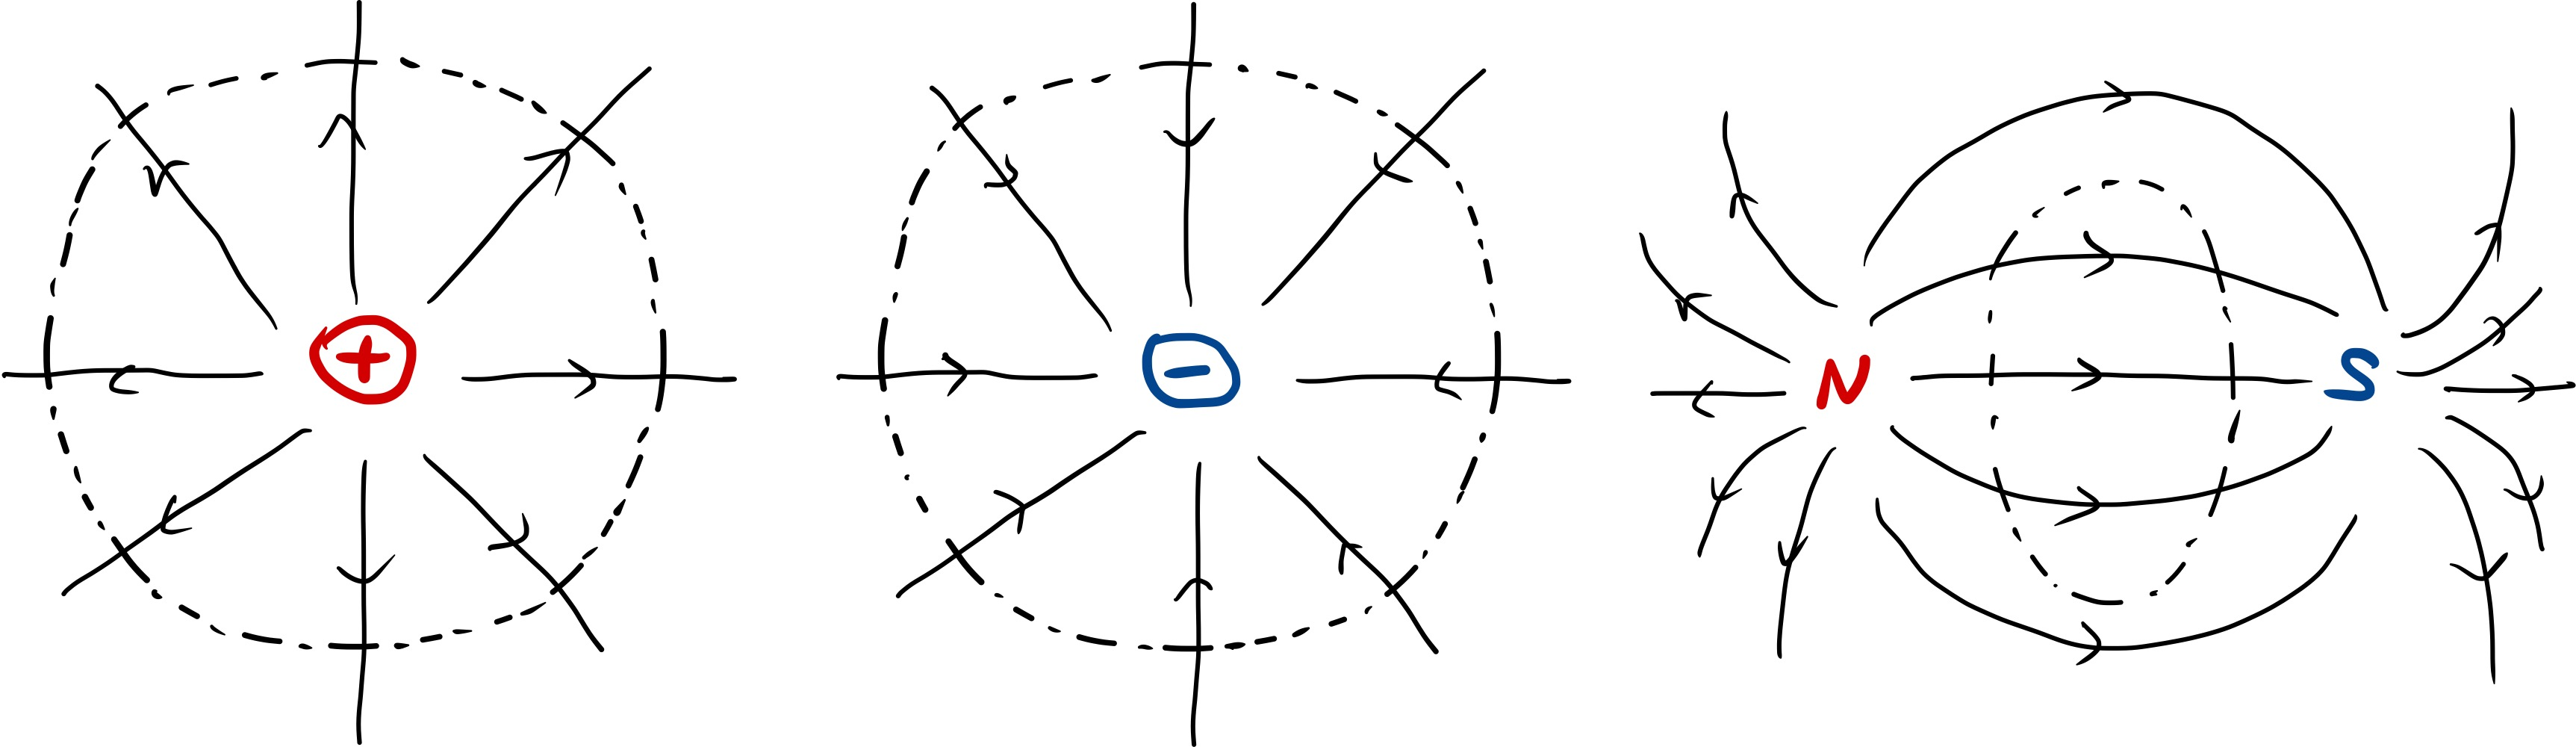
\includegraphics{image-20240125092014626.png}
\caption{image-20240125092014626}
\end{figure}

旋度是一个向量, 因为它的运算方式和叉乘类似, 它描述了每个点上的旋转.
前面这句话有那么一点抽象, 稍微落实一点, 比如向量场描述的是水流,
然后在某个点处放置一个小风车, 风车受到水流的冲击会旋转,
旋度的大小就描述了旋转的快慢, 因为旋度是一个向量,
它的指向反应了向量场旋转的方向 (如下图所示: 利用右手定则,
用四指抓握的方向表示向量场的旋转方向, 拇指的指向便是旋量的指向).

\subsubsection{附录: 通量}

首先要引入一下面积向量, 面积怎么可能用向量来表示呢? 还真可以,
两个向量的叉乘的物理意义可以是,
叉乘结果的大小反应的是它们构成的一个``平行四边形''的面积 (当然,
考虑两个向量微元的叉乘的话就是面积微元了),
叉乘结果的指向是这两个向量所在公共平面的法向 (normal), again
可以利用右手定则确定方向.

\begin{figure}
\centering
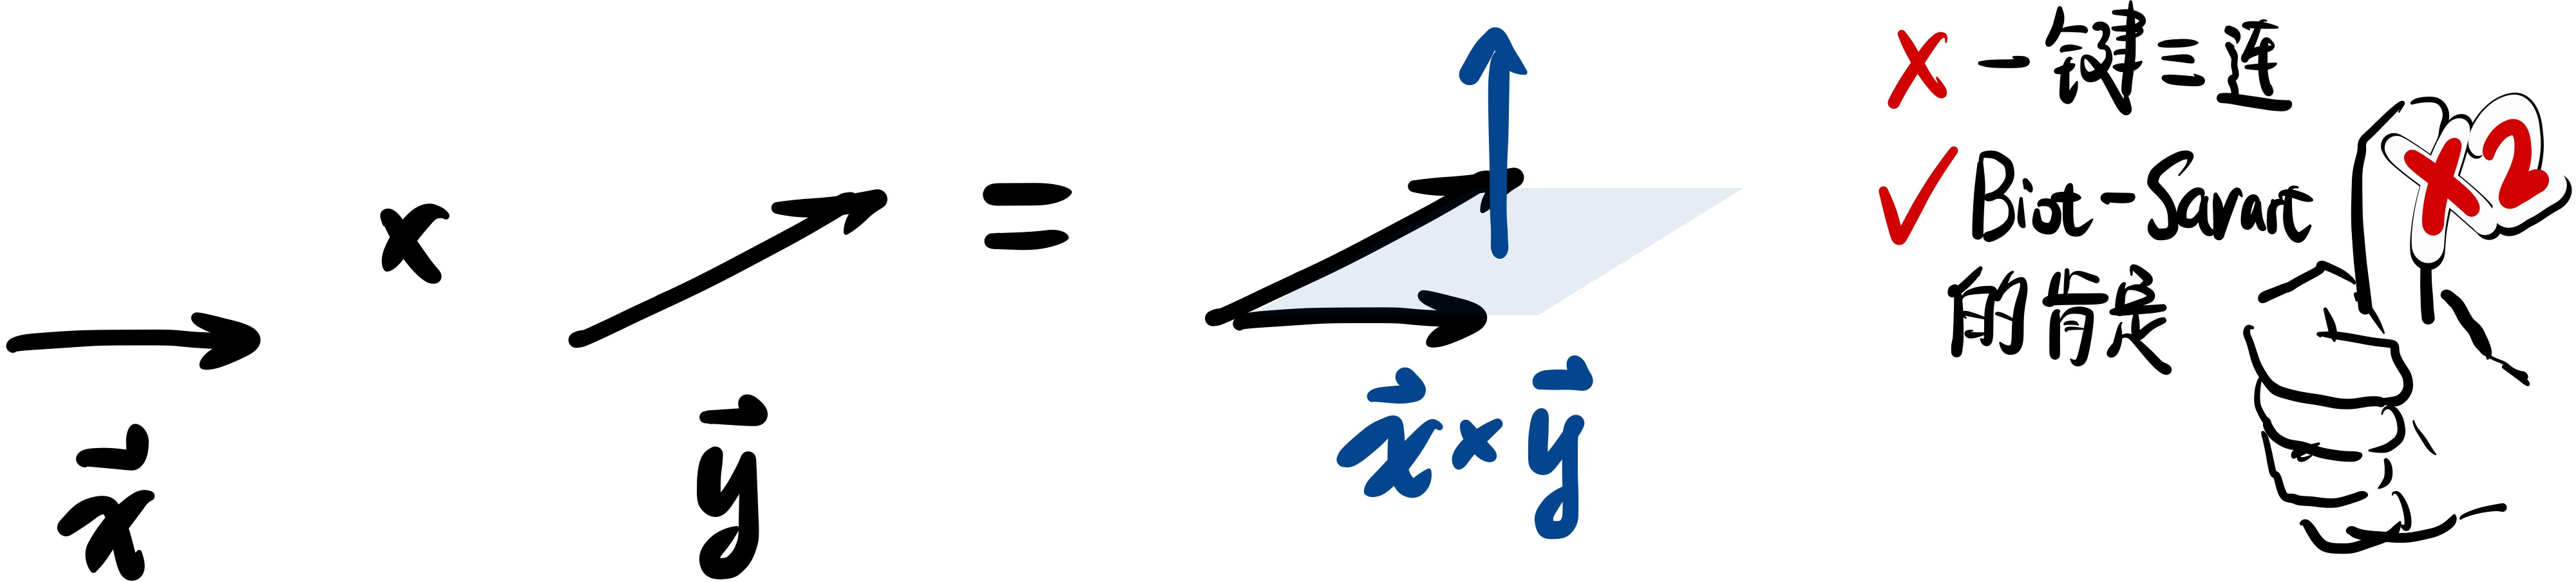
\includegraphics{image-20240125121748817.png}
\caption{image-20240125121748817}
\end{figure}

然后通量计算的就是有多少向量``通过''了一个面积, 在物理里通量常用
\(\Phi\) 表示, 考虑一个向量场 \(\boldsymbol{v}\) 和一块面积
\(\boldsymbol{A}\), 那么通量表示为这个向量场和面积向量的点乘:
\(\Phi=\boldsymbol{v}\cdot\boldsymbol{A}\). 这个结论应该是比较符合直觉 -
intuitive 的: 面积越大, 通量也越大, 向量场越``强'', 通量也越大;
向量场和面积越接近垂直 (也就是向量场的指向和面积向量的指向越一致),
有效通量越大, 对应着公式上, 因为
\(|\Phi|=|\boldsymbol{v}||\boldsymbol{A}|\cos\theta\), \(\theta\) 越接近
\(0\), \(\cos\theta\) 越接近 \(1\), 通量越大.
